\chapter{De quoi sont faits les objets}\label{ch:g1:materials-around-us}

Regarde une table de petit déjeuner. Il y a une cuillère, un verre de
lait, une fourchette, une serviette, un bol, et un pull posé sur le
dossier d'une chaise. Cela fait beaucoup de choses, et chacune est faite
de quelque chose~: la cuillère en bois, la fourchette en métal, le verre
en verre, la serviette en papier, le bol en plastique, le pull en laine.
Une table pleine de choses, faites d'une poignée de matières
différentes seulement. Ce chapitre parle de ces matières.

\begin{omfigure}
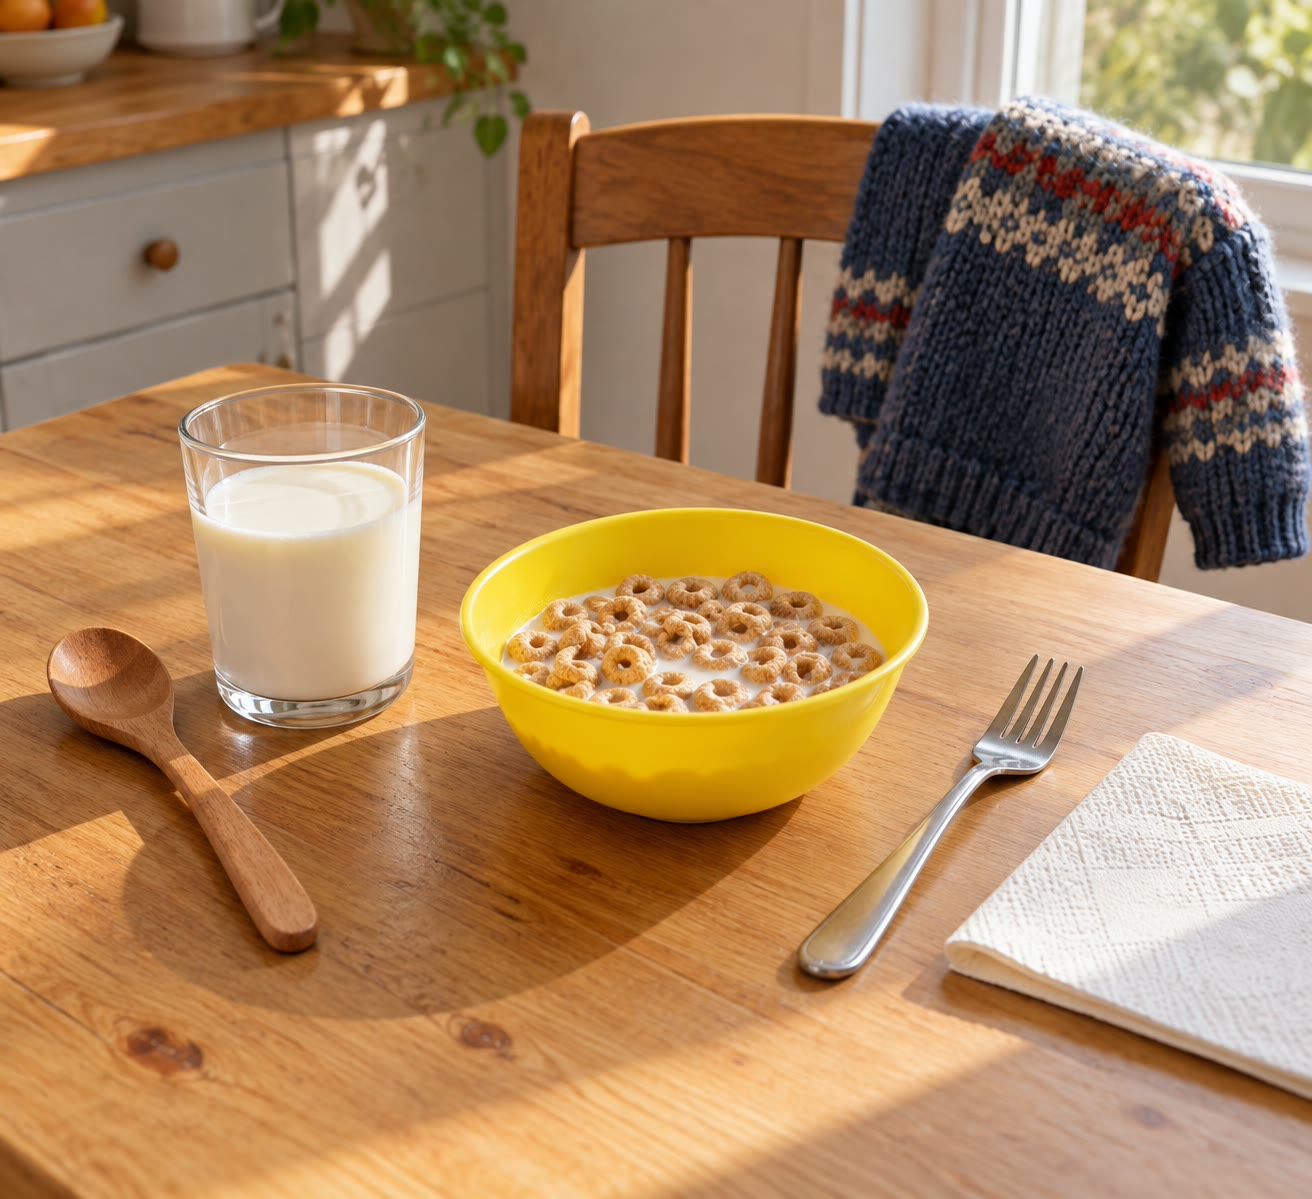
\includegraphics[width=0.62\linewidth]{images/book1/ai/g1-breakfast-table.jpg}

{\small Une table de petit déjeuner~: beaucoup d'\omterm{def:g1:materials-around-us:object}{objets}, faits de quelques matériaux.}
\end{omfigure}

\section{Objets et matériaux}

\begin{definition}[Objet]\label{def:g1:materials-around-us:object}
Un \emph{objet}\index{objet} est une chose que l'on peut voir et
toucher, et souvent prendre en main et utiliser~: une cuillère, une
chaise, un ballon, une fenêtre, une chaussure.
\end{definition}

\begin{definition}[Matériau]\label{def:g1:materials-around-us:material}
Le \emph{matériau}\index{materiau@matériau} d'un \omterm{def:g1:materials-around-us:object}{objet}, c'est ce dont l'\omterm{def:g1:materials-around-us:object}{objet} est
fait. Une cuillère peut être en bois, en métal ou en plastique~: la
cuillère est l'\omterm{def:g1:materials-around-us:object}{objet}, le bois est le matériau.
\end{definition}

\begin{example}[Un objet, trois matériaux]\label{ex:g1:materials-around-us:spoons}
Trois cuillères sont posées côte à côte. Elles ont la même forme et
servent à la même chose~: ce sont donc des \omterm{def:g1:materials-around-us:object}{objets} de la même sorte. Mais
l'une est en bois, l'autre en métal et la troisième en plastique~: trois
matériaux différents.
\end{example}

\begin{omfigure}
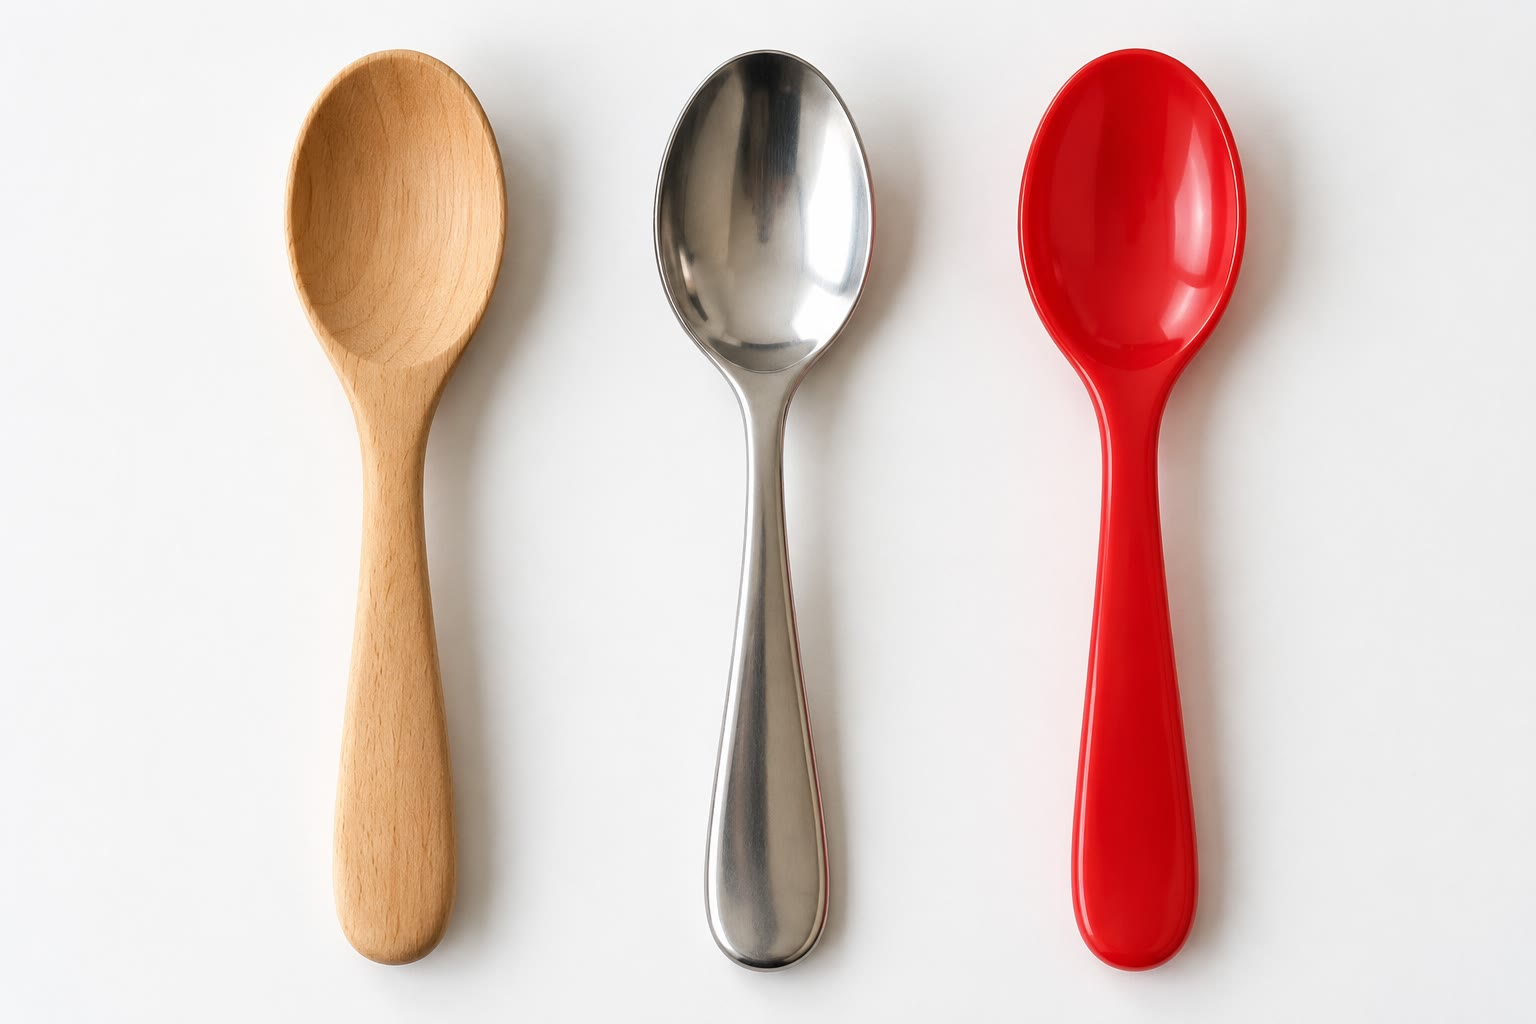
\includegraphics[width=0.55\linewidth]{images/book1/ai/g1-three-spoons.jpg}

{\small Trois cuillères~: le même \omterm{def:g1:materials-around-us:object}{objet}, trois matériaux --- bois, métal
et plastique.}
\end{omfigure}

\begin{example}[Un matériau, beaucoup d'objets]\label{ex:g1:materials-around-us:wood}
Le bois est le \omterm{def:g1:materials-around-us:material}{matériau} d'un crayon, d'une chaise, d'une porte, d'un
petit train et d'une cuillère en bois. Beaucoup d'\omterm{def:g1:materials-around-us:object}{objets} différents
peuvent être faits du même \omterm{def:g1:materials-around-us:material}{matériau}.
\end{example}

\begin{remark}[Des objets faits de plusieurs matériaux]\label{rem:g1:materials-around-us:several}
Beaucoup d'\omterm{def:g1:materials-around-us:object}{objets} sont faits de plus d'un \omterm{def:g1:materials-around-us:material}{matériau}. Une paire de ciseaux
a des lames en métal et des poignées en plastique. Un crayon est en bois
à l'extérieur, avec une mine grise de graphite à l'intérieur. Une
fenêtre est une vitre dans un cadre en bois, en métal ou en plastique.
\end{remark}

\section{Sept matériaux courants}

\begin{proposition}[Des matériaux tout autour de nous]\label{prop:g1:materials-around-us:seven}
La plupart des \omterm{def:g1:materials-around-us:object}{objets} qui nous entourent sont faits de quelques
matériaux courants~:
\begin{itemize}
  \item le \textbf{bois}~: tables, chaises, crayons, portes~;
  \item le \textbf{métal}~: fourchettes, clés, clous, casseroles, vélos~;
  \item le \textbf{verre}~: fenêtres, bocaux, bouteilles, verres~;
  \item le \textbf{plastique}~: bols, bouteilles, jouets, seaux~;
  \item le \textbf{papier} et le carton~: livres, serviettes, boîtes~;
  \item le \textbf{tissu}~: vêtements, rideaux, sacs --- en laine,
        en coton ou en d'autres fils~;
  \item la \textbf{pierre}~: murs, marches, galets, statues.
\end{itemize}
\end{proposition}

\begin{omfigure}
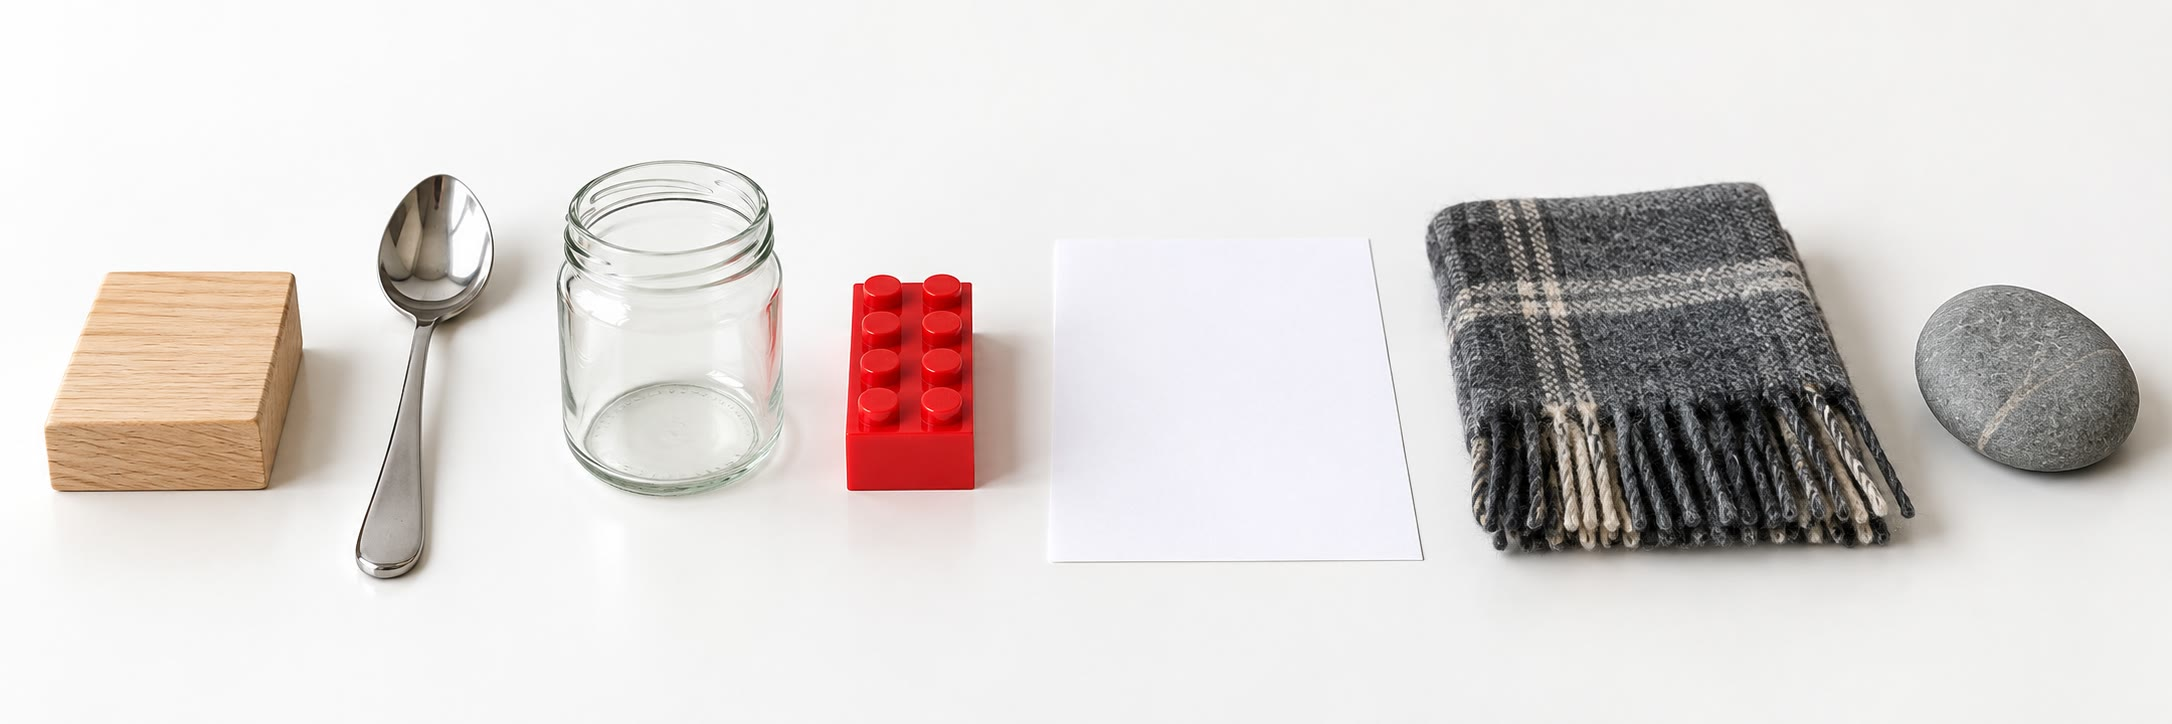
\includegraphics[width=0.75\linewidth]{images/book1/ai/g1-material-samples.jpg}

{\small Sept échantillons, de gauche à droite~: bois, métal, verre,
plastique, papier, tissu (laine) et pierre.}
\end{omfigure}

\begin{remark}[Des noms qui sont aussi des matériaux]\label{rem:g1:materials-around-us:names}
On appelle le récipient dans lequel on boit «~un verre~» parce qu'il
est fait de verre, et une feuille de papier «~un papier~». Le mot de
l'\omterm{def:g1:materials-around-us:object}{objet} et le mot du \omterm{def:g1:materials-around-us:material}{matériau} sont alors les mêmes. Quand on parle de
matériaux, on parle de la matière, pas de l'\omterm{def:g1:materials-around-us:object}{objet}.
\end{remark}

\section{Les propriétés des matériaux}

\begin{definition}[Propriété d'un matériau]\label{def:g1:materials-around-us:property}
Une \emph{propriété d'un matériau}\index{propriete d'un materiau@propriété d'un matériau} est
une chose que l'on peut découvrir sur lui en regardant, en touchant ou
en faisant un essai~: est-il dur ou mou~? Peut-on voir à travers~?
Un aimant l'attire-t-il~? Flotte-t-il sur l'eau ou coule-t-il~?
\end{definition}

\begin{example}[Dur et mou]\label{ex:g1:materials-around-us:hard}
Un galet est dur~: quand on appuie dessus avec le pouce, il ne garde
aucune marque. Une écharpe en laine est molle~: elle se plie dans la
main. Le bois, le métal, le verre et la pierre sont durs~; le tissu et
le papier sont souples et se plient facilement.
\end{example}

\begin{example}[Voir à travers]\label{ex:g1:materials-around-us:see-through}
On voit le jardin à travers une fenêtre~: le verre laisse passer la
lumière, on dit qu'il est \emph{transparent}. On ne voit pas à travers
une porte en bois, un mur de briques ou une casserole en métal.
Certains plastiques sont transparents, comme une bouteille d'eau~;
d'autres non, comme une brique de jeu rouge.
\end{example}

\begin{example}[Attiré par un aimant]\label{ex:g1:materials-around-us:magnet}
Un aimant attire vers lui un trombone en acier, un clou en acier ou une
clé en fer. Il n'attire ni le bois, ni le verre, ni le plastique, ni le
papier, ni le tissu, ni la pierre. Et, chose étonnante, il n'attire pas
tous les métaux~: une canette en aluminium et un fil de cuivre restent
à leur place. Un aimant attire les \omterm{def:g1:materials-around-us:object}{objets} en fer et en acier, qui est
fait surtout de fer.
\end{example}

\begin{omfigure}
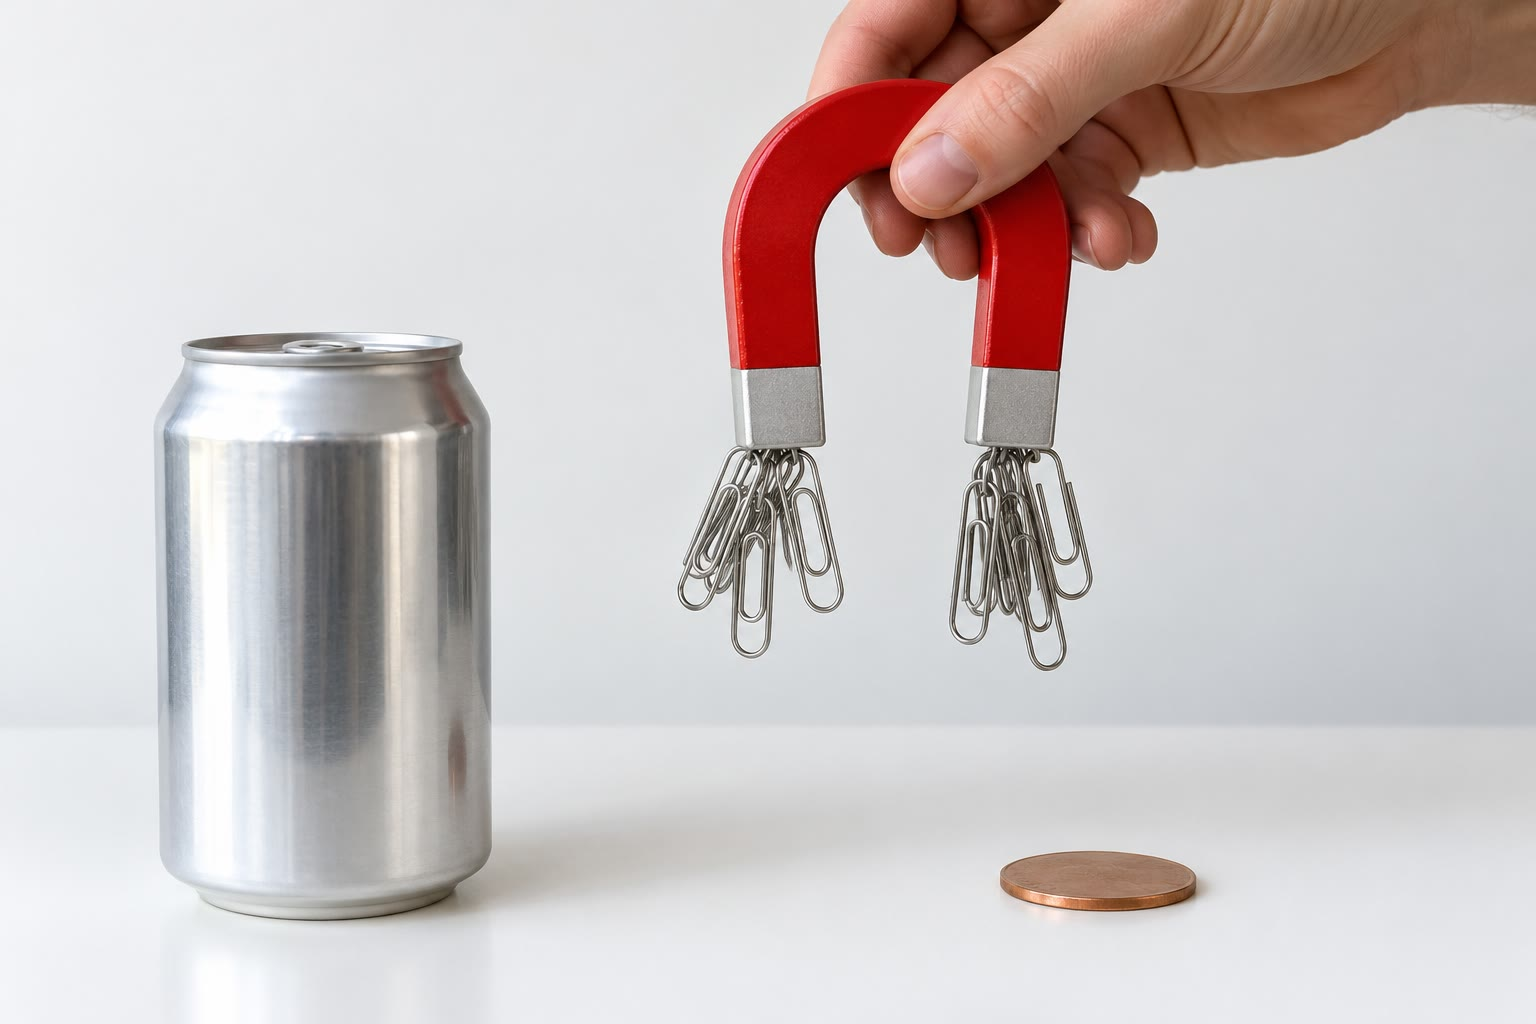
\includegraphics[width=0.55\linewidth]{images/book1/ai/g1-magnet-clips.jpg}

{\small Un aimant soulève des trombones en acier. La canette en
aluminium et le disque de cuivre posés sur la table restent à leur place.}
\end{omfigure}

\begin{example}[Flotter et couler]\label{ex:g1:materials-around-us:float}
Mets quelques \omterm{def:g1:materials-around-us:object}{objets} dans une bassine d'eau. Un bloc de bois et un
bouchon de bouteille en plastique flottent. Un galet, une bille de verre
et un clou en acier coulent au fond. Flotter ou couler, c'est aussi une
propriété du \omterm{def:g1:materials-around-us:material}{matériau} de l'\omterm{def:g1:materials-around-us:object}{objet}.
\end{example}

\begin{omfigure}
\begin{tikzpicture}[font=\small]
  % the basin
  \fill[omWater!80] (0,0) rectangle (9,2.2);
  \draw[omGlass, line width=0.8pt] (-0.1,2.7) -- (0,2.6) -- (0,0) -- (9,0)
    -- (9,2.6) -- (9.1,2.7);
  % floating: wooden block, plastic cap
  \fill[brown!55, draw=brown!70!black] (0.8,2.0) rectangle (2.2,2.5);
  \fill[red!70, draw=red!50!black] (3.7,2.05) rectangle (4.3,2.35);
  % sunk: pebble, marble, nail
  \fill[black!35, draw=black!60] (5.0,0.25) ellipse (0.45 and 0.22);
  \shade[ball color=cyan!40] (6.5,0.2) circle (0.18);
  \fill[black!55] (7.6,0.06) rectangle (8.6,0.14);
  \fill[black!55] (7.52,0.02) rectangle (7.62,0.18);
  % labels
  \node[anchor=south] at (1.5,2.75) {bloc de bois};
  \node[anchor=south] at (4.0,2.75) {bouchon};
  \node[anchor=north] at (5.0,-0.1) {galet};
  \node[anchor=north] at (6.5,-0.1) {bille};
  \node[anchor=north] at (8.1,-0.1) {clou};
  \node[anchor=west, align=left] at (9.3,2.2) {ceux-ci flottent};
  \node[anchor=west, align=left] at (9.3,0.2) {ceux-ci coulent};
\end{tikzpicture}

{\small Dans une bassine d'eau~: le bloc de bois et le bouchon en plastique
flottent~; le galet, la bille de verre et le clou en acier coulent.}
\end{omfigure}

\section{Trier les matériaux}

\begin{method}[Trier selon une seule propriété]\label{met:g1:materials-around-us:sort}
Pour trier un tas d'\omterm{def:g1:materials-around-us:object}{objets}~:
\begin{enumerate}
  \item choisis \textbf{une seule} question, par exemple «~Un aimant
        l'attire-t-il~?~»~;
  \item teste chaque \omterm{def:g1:materials-around-us:object}{objet} et range-le dans le groupe «~oui~» ou dans le
        groupe «~non~»~;
  \item ensuite, si tu veux, trie de nouveau chaque groupe avec une autre
        question.
\end{enumerate}
Une seule question à la fois~: ainsi, chaque \omterm{def:g1:materials-around-us:object}{objet} a exactement une
place.
\end{method}

\begin{omfigure}
\begin{tikzpicture}[font=\small]
  \draw[omDef, line width=1pt] (0,0) circle (2.3);
  \draw[omProp, line width=1pt] (2.4,0) circle (2.3);
  \node[omDef, font=\small\bfseries] at (-0.6,2.65) {en métal};
  \node[omProp, font=\small\bfseries] at (3.0,2.65) {attiré par un aimant};
  \node[font=\footnotesize] at (-1.1,0.35) {canette};
  \node[font=\footnotesize] at (-1.1,-0.35) {fil de cuivre};
  \node[font=\footnotesize] at (1.2,0.6) {clou d'acier};
  \node[font=\footnotesize] at (1.2,0) {clé en fer};
  \node[font=\footnotesize] at (1.2,-0.6) {trombone};
  \node[font=\footnotesize] at (3.5,0) {(rien)};
  \node[anchor=west] at (5.2,0.9) {cuillère en bois};
  \node[anchor=west] at (5.2,0.3) {bille de verre};
  \node[anchor=west] at (5.2,-0.3) {écharpe en laine};
  \node[anchor=west] at (5.2,-0.9) {galet};
\end{tikzpicture}

{\small Deux questions, deux cerceaux. Dans le cerceau bleu~: les \omterm{def:g1:materials-around-us:object}{objets}
en métal. Dans le cerceau orange~: les \omterm{def:g1:materials-around-us:object}{objets} qu'un aimant attire. Dans
les deux cerceaux à la fois~: les \omterm{def:g1:materials-around-us:object}{objets} en fer ou en acier. Hors des
deux~: tout le reste.}
\end{omfigure}

\begin{center}
\small
\begin{tabular}{lccc}
\hline
\omterm{def:g1:materials-around-us:object}{objet} (\omterm{def:g1:materials-around-us:material}{matériau}) & dur~? & transparent~? & attiré par un aimant~? \\
\hline
bloc (bois) & oui & non & non \\
clou (acier) & oui & non & oui \\
bille (verre) & oui & oui & non \\
bouchon (plastique) & oui & non & non \\
feuille (papier) & non & non & non \\
écharpe (laine) & non & non & non \\
galet (pierre) & oui & non & non \\
\hline
\end{tabular}
\end{center}

\section{Le bon matériau pour chaque usage}

\begin{proposition}[Chaque matériau est choisi pour ses propriétés]\label{prop:g1:materials-around-us:choose}
On choisit le \omterm{def:g1:materials-around-us:material}{matériau} d'un \omterm{def:g1:materials-around-us:object}{objet} selon ce que l'\omterm{def:g1:materials-around-us:object}{objet} doit faire~:
\begin{itemize}
  \item une fenêtre doit laisser entrer la lumière~: elle est en verre,
        qui est transparent~;
  \item un imperméable doit arrêter la pluie et se plier~: il est en
        plastique ou dans un tissu que l'eau ne traverse pas~;
  \item une casserole ne doit pas fondre sur la cuisinière~: elle est en
        métal~;
  \item le manche d'une casserole ne doit pas brûler la main~: il est
        souvent en bois ou en plastique dur, qui ne chauffent pas autant
        que le métal~;
  \item un oreiller doit être moelleux~: il est fait de tissu rempli de
        plumes ou de fibres.
\end{itemize}
\end{proposition}

\begin{example}[Un bateau]\label{ex:g1:materials-around-us:boat}
Un bateau-jouet doit flotter. Il peut être en bois ou en plastique. Un
bateau taillé dans un bloc de pierre coulerait tout de suite.
\end{example}

\begin{remark}[Le verre cassé]\label{rem:g1:materials-around-us:glass}
Le verre est dur, mais il se casse, et ses morceaux sont coupants. Quand
un verre se casse, c'est un adulte qui ramasse les morceaux.
\end{remark}

\section{Exercices}

\begin{exercise}[$\star$]\label{exo:g1:materials-around-us:1}
Une chaise est-elle un \omterm{def:g1:materials-around-us:object}{objet} ou un \omterm{def:g1:materials-around-us:material}{matériau}~? Le bois est-il un \omterm{def:g1:materials-around-us:object}{objet} ou
un \omterm{def:g1:materials-around-us:material}{matériau}~?
\end{exercise}

\begin{exercise}[$\star$]\label{exo:g1:materials-around-us:2}
Nomme le \omterm{def:g1:materials-around-us:material}{matériau} de chaque \omterm{def:g1:materials-around-us:object}{objet}~: une vitre, un clou, un galet, un
livre, une chaussette.
\end{exercise}

\begin{exercise}[$\star$]\label{exo:g1:materials-around-us:3}
Donne deux \omterm{def:g1:materials-around-us:object}{objets} en bois et deux \omterm{def:g1:materials-around-us:object}{objets} en plastique.
\end{exercise}

\begin{exercise}[$\star$]\label{exo:g1:materials-around-us:4}
Trouve l'intrus et dis pourquoi~: une cuillère en bois, une fourchette
en métal, une cuillère en plastique, une chaise en bois. (Regarde les
matériaux.)
\end{exercise}

\begin{exercise}[$\star$]\label{exo:g1:materials-around-us:5}
Quel \omterm{def:g1:materials-around-us:material}{matériau} laisse voir à travers lui~: le bois, le verre ou la pierre~?
\end{exercise}

\begin{exercise}[$\star$]\label{exo:g1:materials-around-us:6}
On approche un aimant d'un clou en acier, d'une bille de verre et d'un
bloc de bois. Lequel attire-t-il~?
\end{exercise}

\begin{exercise}[$\star$]\label{exo:g1:materials-around-us:7}
Regarde la figure de la bassine. Combien d'\omterm{def:g1:materials-around-us:object}{objets} flottent~? Combien
coulent~?
\end{exercise}

\begin{exercise}[$\star$]\label{exo:g1:materials-around-us:8}
Une paire de ciseaux a des lames et des poignées. En quel \omterm{def:g1:materials-around-us:material}{matériau} est
chaque partie~? Une paire de ciseaux est-elle faite d'un seul \omterm{def:g1:materials-around-us:material}{matériau}
ou de deux~?
\end{exercise}

\begin{exercise}[$\star$]\label{exo:g1:materials-around-us:9}
Regarde la figure des deux cerceaux. Dans quel cerceau est la canette~?
Pourquoi n'est-elle pas dans le cerceau orange~?
\end{exercise}

\begin{exercise}[$\star\star$]\label{exo:g1:materials-around-us:10}
Pourquoi les fenêtres sont-elles en verre et pas en bois~?
\end{exercise}

\begin{exercise}[$\star\star$]\label{exo:g1:materials-around-us:11}
Sam veut trier ces 8 \omterm{def:g1:materials-around-us:object}{objets} avec la question «~Un aimant l'attire-t-il~?~»~:
un clou en acier, un trombone, un galet, une cuillère en bois, une clé en
fer, une canette, une bille de verre, une chaussette en laine. Combien
d'\omterm{def:g1:materials-around-us:object}{objets} vont dans le groupe «~oui~»~? Combien dans le groupe «~non~»~?
\end{exercise}
